

Assim,
\begin{equation}
P(a < u < b) = 1 - \alpha
\end{equation}

\[
\therefore \quad P\left(a < \frac{T}{\theta} < b\right) = 1 - \alpha 
\quad \therefore \quad P\left(\frac{1}{b} < \frac{\theta}{T} < \frac{1}{a}\right) = 1 - \alpha
\]

\[
\therefore \quad P\left(\theta \in \left(\frac{T}{b}, \frac{T}{a}\right)\right) = 1 - \alpha, \quad e
\]

\begin{equation}
IC_{1-\alpha}(\theta) = \left(b^{-1} X_{n:n}, \; a^{-1} X_{n:n}\right)
\end{equation}

\textbf{Q(56)} Sejam $X_1, \ldots, X_n$ uma amostra de $X \sim N(\mu, \sigma^2)$ com $\mu \in \mathbb{R}$ desconhecido e $\sigma^2 > 0$ conhecido. Encontre o IC bilateral com $1 - \alpha$ de confiança para $\mu$.

\textbf{Solução} \\
De discussões anteriores $T = \bar{X}_n$ é uma estatística suficiente mínima para $\mu$ e $T \sim N(\mu, \sigma^2/n)$. \\
Assim, $X_i$'s e $T$ pertencem a uma família locação. \\
Note que
\begin{equation}
U = \frac{\bar{X}_n - \mu}{\sigma / \sqrt{n}} \sim N(0,1)
\end{equation}
é um pivô para $z_{\alpha/2}$, logo temos
\begin{equation}
P\left(-z_{\alpha/2} < U < z_{\alpha/2}\right) = 1 - \alpha
\end{equation}

\[
\therefore \quad P\left(-z_{\alpha/2} < \frac{\bar{X}_n - \mu}{\sigma / \sqrt{n}} < z_{\alpha/2}\right) = 1 - \alpha
\]

\[
\therefore \quad P\left(\mu \in \left(\bar{X}_n + \frac{\sigma}{\sqrt{n}}(-z_{\alpha/2}), \; \bar{X}_n + \frac{\sigma}{\sqrt{n}} z_{\alpha/2}\right)\right) = 1 - \alpha
\]

\begin{center}
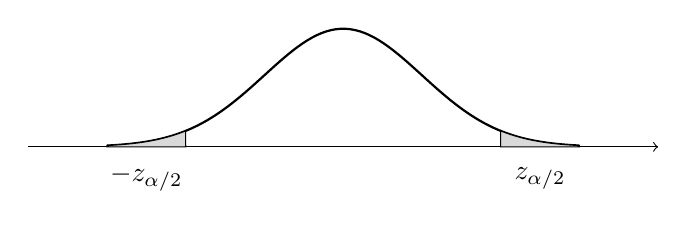
\begin{tikzpicture}
\draw[->] (-4,0) -- (4,0);
\draw[thick] plot[domain=-3:3,samples=100] (\x,{1.5*exp(-\x*\x/2)});
\draw[fill=gray!30] (-3,0) -- plot[domain=-3:-2,samples=100] (\x,{1.5*exp(-\x*\x/2)}) -- (-2,0) -- cycle;
\draw[fill=gray!30] (2,0) -- plot[domain=2:3,samples=100] (\x,{1.5*exp(-\x*\x/2)}) -- (3,0) -- cycle;
\node at (-2.5,-0.4) {$-z_{\alpha/2}$};
\node at (2.5,-0.4) {$z_{\alpha/2}$};
\end{tikzpicture}
\end{center}
